% This document is part of the transientdict project.
% Copyright 2013 the authors.

\documentclass[12pt]{emulateapj}
\usepackage{xspace}
\usepackage{graphicx}
%\usepackage{epsfig}
\usepackage{times}
\usepackage{natbib}
\usepackage{amsfonts}
\usepackage{amsmath}
\usepackage{amsbsy}
\usepackage{bm}
\usepackage{hyperref}
\usepackage{url}
%\usepackage{subfigure}
\usepackage{microtype}
\usepackage{rotating}
\usepackage{booktabs}
\usepackage{threeparttable}
\usepackage{tabularx}
\usepackage{subcaption}
\usepackage{minted}


%\usepackage{longtable}%\usepackage[stable]{footmisc}
%\usepackage{color}
%\bibliographystyle{apj}

% MB: I added xspace so that we don't have to use '\ ' after the commands
% For commands that may or may not stay inside a math environment, we can 
% also use \ensuremath
\newcommand{\project}[1]{\textsl{#1}\xspace}
\newcommand{\fermi}{\project{Fermi}\xspace}
\newcommand{\rxte}{\project{RXTE}\xspace}
\newcommand{\given}{\ensuremath{\,|\,}}
\newcommand{\dd}{\ensuremath{\mathrm{d}}}
\newcommand{\counts}{\ensuremath{y}}
\newcommand{\pars}{\ensuremath{\theta}}
\newcommand{\mean}{\ensuremath{\lambda}}
%\newcommand{\likelihood}{\ensuremath{{\mathcal L}}}
\newcommand{\Poisson}{\ensuremath{{\mathcal P}}}
\newcommand{\Uniform}{\ensuremath{{\mathcal U}}}
\newcommand{\bg}{\ensuremath{\mathrm{bg}}}
\newcommand{\word}{\ensuremath{\phi}}
\newcommand{\zsq}{\ensuremath{Z^2_n}}
\newcommand{\stingray}{\mintinline{python}{stingray}\xspace}
\newcommand{\python}{\texttt{Python}\xspace}
\newcommand{\astropy}{\texttt{astropy}\xspace}
\newcommand{\lightcurve}{\mintinline{python}{Lightcurve}\xspace}
\newcommand{\eventlist}{\mintinline{python}{EventList}\xspace}
\newcommand{\crossspectrum}{\mintinline{python}{Crossspectrum}\xspace}
\newcommand{\powerspectrum}{\mintinline{python}{Powerspectrum}\xspace}
\newcommand{\likelihood}{\mintinline{python}{Likelihood}\xspace}
\newcommand{\posterior}{\mintinline{python}{Posterior}\xspace}
\newcommand{\parest}{\mintinline{python}{ParameterEstimation}\xspace}


\usemintedstyle[python]{friendly}
%\setminted[python]{}
%\setmintedinline[python]{}

\newcommand{\hendrics}{\texttt{HENDRICS}\xspace}
\newcommand{\dave}{\texttt{DAVE}\xspace}


%\newcommand{\bs}{\boldsymbol}

\begin{document}

\title{\stingray: A Modern \python\ Library For Spectral Timing}

\author{D. Huppenkothen\altaffilmark{1, 2}, M. Bachetti\altaffilmark{4}, A. Stevens\altaffilmark{}, OTHER CO-AUTHORS!}
 
\altaffiltext{1}{DIRAC Institute, Department of Astronomy, University of Washington, 3910 15th Ave NE, Seattle, WA 98195}
  \altaffiltext{2}{E-mail: dhuppenk@uw.edu}
\altaffiltext{3}{INAF-Osservatorio Astronomico di Cagliari, via della Scienza 5, I-09047 Selargius (CA), Italy}
\altaffiltext{4}{}
\altaffiltext{5}{}
\altaffiltext{6}{}


\begin{abstract}
% This abstract could be more exciting, I think.
This paper describes the design, implementation and usage of \stingray, a library in \python built to perform time series analysis and related tasks on astronomical light curves. 
Its core functionality comprises a large range of Fourier analysis techniques commonly used in Spectral Timing, as well as extensions for analysing pulsar data, simulating data sets, and statistical modelling. 
Its modular build allows for easy extensions and we aim for the library to be a platform for future development. 
Here, we describe its Python classes and functions in detail, as well as give practical example using astronomical data sets. 
The code is well-tested, with a test coverage of currently 95\%.

\end{abstract}

\keywords{methods:statistics}

\section{Introduction}

Variability is one of the key diagnostics in understanding the underlying physics of the dynamics and emission processes from astronomical objects. 
The detection of periodic variations in the radio flux of certain objects has led to the ground-breaking discovery of pulsars. Similarly, accurately describing of dips in stellar light curves has led to the discovery of thousands of exoplanets. 
In high-energy astrophysics, particularly the study of black holes and neutron stars, the scientific developments of recent years have brought a growing understanding that time and wavelength are intricately linked. 
Different spectral components react differently to changes in accretion rate and dynamics, leading to time lags, correlated variability and higher-order effects. 
This has led to the study of accretion disks, in particular those of Active Galactic Nuclei (AGN), via reverberation mapping. 
Understanding how the emission at various wavelengths changes with time is crucial for testing and expanding our understanding of General Relativity in the strong gravity limit, the dense matter equation of state and other fundamental questions in astrophysics.

\section{Vision}

Despite decades of research, the field is fragmented in terms of software; there is no commonly accepted, up-to-date framework for the core data analysis tasks involved in (spectral) timing. Code is generally siloed within groups, leading to a general lack of reproducibility of scientific results. Additionally, the lack of fully open-source tools constitutes a significant barrier to entry for researchers new to the field, since it effectively requires anyone not part of collaborations with an existing private code base to write their own software from scratch. 
The NASA library \texttt{xronos} is, to our knowledge, the only significant open-source library in this field, and has several shortcomings. 
In particular, it performs only a few of the most basic tasks, and it has not been maintained since 2004. 
Here, we introduce \stingray, a lightweight library built entirely in \python and based on \astropy functionality, to address the lack of well-tested, well-documented software for spectral timing. 
\stingray aims to make many of the core Fourier analysis tools used in timing analysis available to a large range of researchers while providing a common platform for new methods and tools as they enter the field. 
It includes the most relevant functionality in its core package, while extending that functionality in its subpackages in several ways, allowing for easy modeling of light curves and power spectra, simulation of synthetic data sets and pulsar timing. 

Its primary idea is to provide time series analysis methods in an accessible, well-tested way, built as a series of modules in an object-oriented way. In practice, data 
analysis requirements are varied and depend on the type of data, the wavelength the observation was taken at, and the object being observed. With this in mind, 
\stingray does not aim to provide full data analysis workflows; rather, it provides the core building blocks for users to build such workflows themselves, based on the specific data analysis requirements of their source and observation. 
The modularity of its classes allows for easy incorporation of existing \stingray functionality into larger data analysis workflows and pipelines, while being easily extensible for cases that the library currently does not cover. 

\stingray is designed to be used both as a standalone package, but is also at the core of two other software packages currently under development: \hendrics \citep{hendrics} provides pre-built data analysis workflows using \stingray core functionality. These workflows are accessible from the command line and are provided for some common data types and data analysis tasks. \dave\footnote{\url{https://github.com/StingraySoftware/dave}} on the other hand, provides a Graphical User Interface on top of \stingray to allow for easy interactive exploratory data analysis.
 
As of v0.1, it includes basic functionality depends exclusively on \texttt{numpy} \citep{numpy}, \texttt{scipy} \citep{scipy} and \texttt{astropy} \citep{astropy}, with optional plotting functionality supplied by \texttt{matplotlib} \citep{matplotlib} and \texttt{corner} \citep{corner}, and optional sampling methods by \texttt{emcee} \citep{emcee}. [ADD OTHER OPTIONAL DEPENDENCIES HERE!].

This paper describes \stingray v0.1, released on 2018-02-12. 
As with most open-source packages, \stingray is under continuous development and welcomes contributions from the community.
The paper layout is as follows: 
In Section \ref{sec:general_package}, we describe the general package structure. 
In Section \ref{sec:core}, we detail the package's core functionality in Fourier analysis and introduce basic classes for storing light curves and Fourier spectra of various types. 
In Section \ref{sec:modeling}, we extend this core functionality with \stingray's modeling framework and in Section \ref{sec:simulator}, we show how users can easily simulate data sets from models. 
Section \ref{sec:pulsar} lays out the functionality for analysing pulsar data, and Sections \ref{sec:hendrics} and \ref{sec:dave} details existing connections to the command-line interface and a graphical user interface, respectively, which currently being developed in parallel to \stingray. 
Finally, in Sections \ref{sec:development} and \ref{sec:future} we lay out the development process, testing and documentation environments as well as our future development plans. 
In each section, we present examples of the functionality described based on real-world data sets.

\section{General Package Framework}
\label{sec:general_package}

\stingray separates out core functionality from several more specialized tasks based on those core classes and functions. Constructs related to data products as well as transformations of the data (e.g.\ power spectra, cross spectra, time lags, and other spectral timing products) are considered core functionality, as are some utility functions and classes, for example related to Good Time Interval calculations. 

Current functionality in subpackages includes a framework to allow for the parametric modelling of light curves and Fourier products, simulations of spectral timing products from power spectra, and period searches in pulsars.


\section{Core Functionality}
\label{sec:core}

\stingray imports its core functions and classes from the top level package. 
These classes define the basic data structures such as light curves and cross- as well as power spectra that are used in much of the higher-level functionality provided in the sub-packages. 
Additionally, it incorporates a large range of utilities for dealing with Good Time Intervals (GTIs) as well as input and output of data sets. 

\subsection{The \texttt{Lightcurve} class}
\label{sec:lightcurve}

We expect \stingray to be used largely on data sets of two forms: (1) event data (i.e. recordings of arrival times of individual photons) or (2) binned light curves. 
The majority of methods in \stingray use binned light curves, which we thus currently consider the default format. The \lightcurve class defines a basic data structure to store binned light curves. For binned data, the class can simply be invoked supplying time stamps and the corresponding flux values (and optionally uncertainties on the flux measurements):

\begin{minted}{python}
lc = Lightcurve(time, counts, err, 
		       input_counts=True, 
		       gti=None, 
		       err_dist='poisson', 
		       mjdref=0, dt=None)
\end{minted}

where \texttt{counts} corresponds to the flux per bin (or the number of photon counts per bin in the photon counting case), \texttt{err} are the flux uncertainties and \verb|input_counts| should be set to \texttt{True} if the input is in flux per bin (as opposed to flux per second). While it is possible to input GTIs, they will not by default be applied to the light curve itself, but propagated to classes and functions that take \lightcurve objects as input and make use of the GTIs stored in the object. There is, however, a method that splits a light curve into several \lightcurve objects, one for each contiguous good time interval. For unevenly sampled data or cases where gaps exist in the data, the internal algorithm for determining the time resolution \texttt{dt} might not always be correct; in these cases, it can help to input a reference time resolution manually.

For event data, a static method exists that will take the time stamps of events as well as a time resolution and create a light curve using \texttt{numpy.histogram}:

\begin{minted}{python}
lc = make_lightcurve(toa, dt, tseg=None, 
		     tstart=None, 
		     gti=None,
		     mjdref=0,
		     use_hist=False)
\end{minted}

Here, \texttt{toa} should be a list or array of times of arrivals of the events and \texttt{dt} the time resolution of the binned light curve. By default, the light curve start with the arrival of the first photon and end with the arrival of the last photon. Optionally, if the observation or segment begins before the arrival time of the first event and/or ends after the arrival time of the last event, one may optionally include a start time \texttt{tstart} and a total duration \texttt{tseg} for the creation of the regular time grid. 

Beyond providing a basic data structure for light curves and a creation mechanism out of event data, \stingray implements a range of operations acting on these objects. It overrides several standard operations such as the \texttt{+} operator \verb|__add__| and the \texttt{-} operator \verb|__sub__|, allowing to efficiently add and subtract light curves from one another. In either case, the addition and subtraction will operate on the \texttt{counts} attribute, and derivative attributes such as \verb|count_rate| and \texttt{err} will be automatically be recalculated. Similarly overloaded operations are the built-in function \verb|__len__|, which will return the number of time bins in the light curve, and \verb|__neg__|, which will invert the values in the \texttt{counts} attribute.

Other functionality on light curves includes rebinning to a new time resolution, which must be lower than the previous time resolution (i.e.\ interpolation is not implemented). 
\lightcurve objects can also be joined, truncated and sorted by time or counts. Finally, \stingray implements basic methods for plotting (useful for a quick look at the data), as well as reading and writing into various formats (currently FITS, HDF5 and ASCII).

\subsection{The \texttt{Events} class}

At short wavelengths, data is largely recorded as \textit{photon events}, where arrival times at the detector are recorded for each photon independently, along with a number of other properties of the event (for example an energy channel in which the photon was recorded in, which can be transformed to a rough estimate of the energy of the original photon arriving at the detector).

\stingray implements a basic class \eventlist that acts as a container for data sets of these types. Even for a single instrument, there are often multiple data formats and types of data recorded, resulting in a plethora of data formats and internal schema to how data is stored within the FITS files distributed to the community. 
\stingray implements a basic \eventlist class that acts as a container for basic event data, but does not aim to encompass all current data types of all current (and future) instruments entirely. Instead, it aims to abstract away from instrument-specific idosyncrasies as much as possible and remain mission-agnostic. In its basic form, it takes arrays with time stamps and optionally corresponding photon energies as input, and implements a set of basic methods. Similarly to \lightcurve, it provides basic input/output (I/O) functionality in the form of \texttt{read} and \texttt{write} methods as well as a method to join event lists, which can be particularly useful when data is recorded in several independent detector, as is common for several current and future X-ray missions. The \verb|to_lc| method provides straightforward connection to create a \lightcurve directly out of an \eventlist object. In return, it is possible to create an \eventlist out of a \lightcurve object using the \verb|from_lc|. The latter will create $N_i$ events, each with a time stamp equation to the time bin $t_i$, where $N_i$ is the number of counts in bin $i$ (event lists are, by their very definition only a useful data product if the light curve used to simulate comes from photon counting data in the first place). 
It is possible to simulate more physically meaningful photon events from a given light curve and energy spectrum using the \verb|simulate_times| and \verb|simulate_energies| methods, which employ a combination of interpolation and rejection sampling to accurately draw events from the given light curve and spectrum.


\subsection{Cross Spectra and Power Spectra}
\label{sec:csps}

The cross spectrum and the power spectrum\footnote{TEXT ABOUT DIFFERENCE BETWEEN PERIODOGRAM AND POWER SPECTRUM} are closely related (for a pedagogical introduction into Fourier analysis, see \citealt{vanderklis1989}; see also \citealt{uttley2014} for a recent review of spectral timing techniques). Computing the cross spectrum requires two evenly sampled time series $\mathbf{y}_1$ and $\mathbf{y}_2$ taken simultaneously at exactly the same time bins. Under this assumption, one may then compute the discrete Fourier transform of each time series, $\mathcal{F}_1$ and $\mathcal{F}_2$ independently, and multiple the $\mathcal{F}_1$ with $\mathcal{F}*_2$, i.e. the Fourier transform of the first time series with the \textit{complex conjugate} of the Fourier transform of $\mathbf{x}_2$. 

Because the power spectrum is defined as the square of the real part of the Fourier amplitudes of a single, evenly sampled time series, it can be formulated as the special case of the cross spectrum where $\mathbf{x}_1 = \mathbf{x}_2$. In \stingray, we implement a class \crossspectrum, which takes two \lightcurve objects as input and internally calculates the complex cross spectrum in one of a number of common normalizations.  Because many of the internal calculations are the same, the class \powerspectrum is implemented as a subclass of \crossspectrum, but takes only a single \lightcurve object instead of two. 

There are several popular normalizations for the real part of the cross spectrum as well as the power spectrum implemented in \stingray: the popular Leahy normalization \citep{leahy1983} is defined such that for simple white noise, the power spectrum will follow a $\chi^2$ distribution with $2$ degrees of freedom around a mean value of $2$. It is particularly useful for period searches, because the white noise level is well understood and always the same (but be aware that detector effects like dead time can distort the power spectrum in practice [REF BACHETTI]).
For light curves with complex variability patterns, and especially understanding how these patterns contribute to the overall variance observed, the \textit{fractional rms normalization}\citep{belloni1990,miyamoto1992}  or the \textit{absolute rms normalization}[REF?] may be more appropriate choices. 

These normalizations can be set when instantiating a \crossspectrum or \powerspectrum object using the keyword argument \texttt{norm}, e.g.
\begin{figure*}[htbp]
\begin{center}
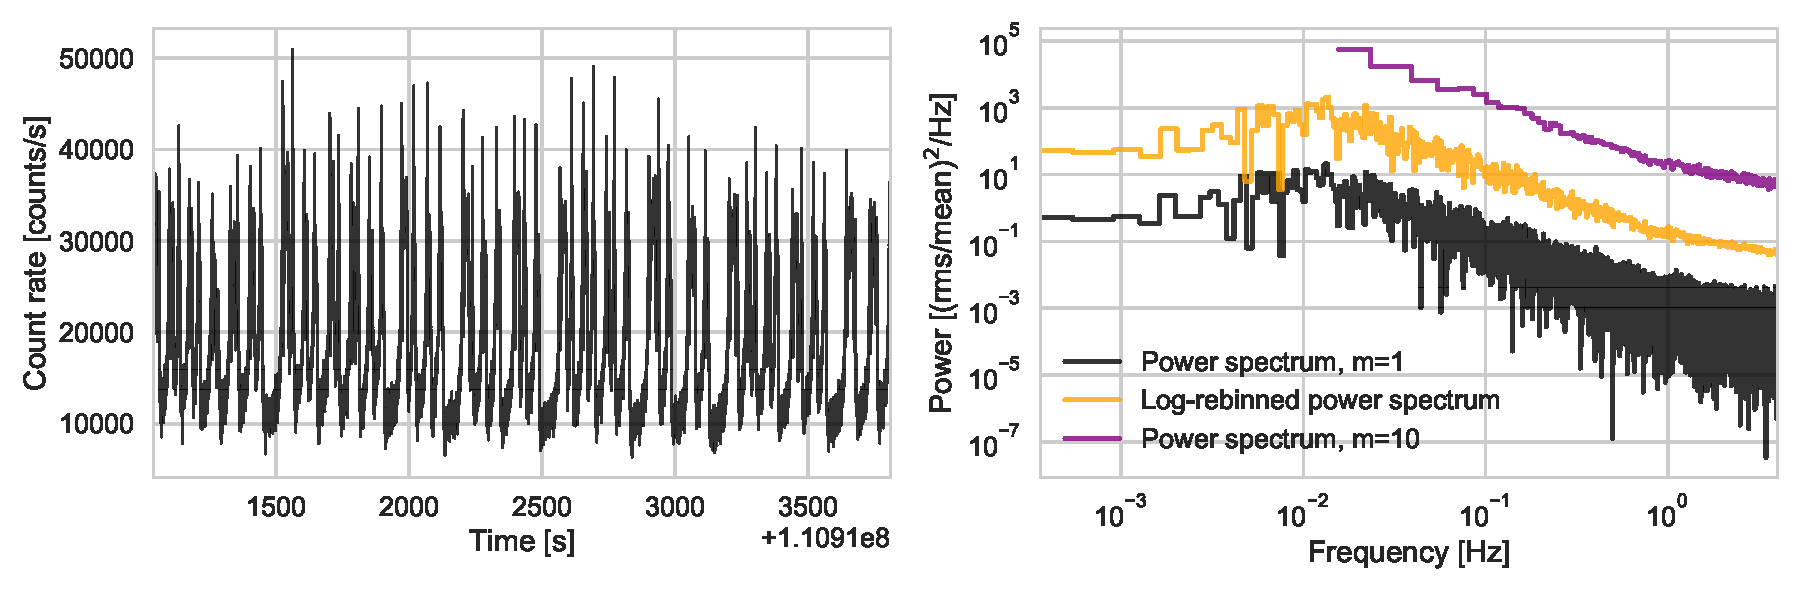
\includegraphics[width=\textwidth]{example_lc_ps.pdf}
\caption{Left panel: An example light curve of the black hole X-ray binary GRS 1915+105, taken with the \textit{Rossi} X-ray Timing Explorer's Proportional Counter Array (PCA) in the $\rho$ state [REF]. Right panel: we show the power spectrum calculated from the light curve in the left panel (black), as well as a version of the same power spectrum that has been logarithmically binned in frequency space (orange) and an averaged power spectrum calculated from $43$ segments of $256\,\mathrm{s}$ duration (purple). The log-rebinned and averaged power spectrum are normalized in the same way as the single-segment power spectrum, but arbitrarily shifted on the y-axis for clarity of comparison.}
\label{fig:psd}
\end{center}
\end{figure*}

\begin{minted}{python}
ps = Powerspectrum(lc, norm="leahy")
\end{minted}

\noindent Setting \mintinline{python}{norm="none"} will return the raw, unnormalized powers. The classes \crossspectrum and \powerspectrum share most of the implemented methods, except where otherwise noted. Both classes include methods to rebin cross- and power spectra. Linear rebinning is implemented analogously to the method in class \lightcurve. Additionally, logarithmic binning is implemented in the method \mintinline{python}{rebin_log} in such a way that the bin width at a given frequency increases a fraction of the previous bin width:

\[
d\nu_{i+1} = d\nu_{i} (1 + f) \; ,
\]

\noindent where $f$ is some constant factor by which the frequency resolution increases, often $f = 0.01$. 

In the case of the cross spectrum, it is also possible to calculate the time lag, defined as

\[
\tau_j = \frac{\phi_j}{2\pi\nu_j} \; 
\]

\noindent for a phase angle $\phi_j$ derived from the imaginary component of the complex cross spectrum, and a mid-bin frequency $\nu_j$. Similarly, it is possible to calculate the coherence \citep{vaughan1997,nowak1999} from the cross spectrum, defined as 

\begin{equation}
c_j = \frac{C_{xy,j}}{C_{x,j} C_{y,j}} \; . 
\end{equation}

\noindent Here, $C_{xy,j}$ corresponds to the real part of the unnormalized cross spectrum, and $C_{x,j}$ and $C_{y,j}$ correspond to the analogous squared amplitudes of the power spectrum for each individual light curve. 

Classical period searches are often formulated as outlier detection problems from an expected statistical distribution. Assuming the signal is sufficiently coherent such that all of the signal power is concentrated in one bin, one may calculate the chance probability that an observed power was generated by statistical fluctuations alone. The distribution for power spectra is well known: For a Leahy-normalized spectrum, the powers are distributed following a $\chi^2$ distribution around a mean of $2$ in the case of pure white noise, and following a $\chi^2$ distribution around an underlying power spectral shape for other stationary stochastic processes. In the white noise case, the equations to accurately calculate a $p$-value of rejecting the hypothesis that a given outlier in the power spectrum was generated by white noise was defined in \citep{Groth1975}, and can be calculated for one or multiple powers in a \powerspectrum object using the \verb|classical_significances| method:

\begin{minted}{python}
pvals = ps.classical_significances(threshold=0.01, 
                      trial_correction=True)
\end{minted}

\noindent where the \mintinline{python}{threshold} keyword argument sets the minimum threshold below which $p$-values will be reported, and \mintinline{python}{trial_correction} is a boolean keyword that sets whether the threshold will be corrected for the number of trials (i.e. the number of frequencies in the power spectrum). 
The return variable \mintinline{python}{pvals} provides the $p$-value for each power that falls below the (trial-corrected) threshold as well as the index of that power in the original array in the \powerspectrum object.
Note that the cross spectrum does not follow the same distribution \citep{huppenkothen2017}, and the recently derived statistical distributions for this case will be implemented in a future version of \stingray. 

In many practical applications, users may wish to average power- or cross spectra from multiple light curve segments in order to suppress statistical noise. This can easily be done with the appropriate classes \texttt{AveragedPowerspectrum} and \texttt{AveragedCrossspectrum}, which take a \lightcurve object or list of \lightcurve objects as an input and will compute averaged Fourier products for a given length of segment. Both are subclasses of \crossspectrum, and either inherit or override many of the methods relevant for those classes as well:

\begin{minted}{python}
# segment size in same time units 
# as light curve object
seg_size = 256.0
# compute averaged power spectrum
avg_ps = AveragedPowerspectrum(lc, seg_size, 
                               norm="frac")
\end{minted}

\noindent An example of the kinds of products produced by the functions above is given in Figure \ref{fig:psd}.


\begin{figure}[htbp]
\begin{center}
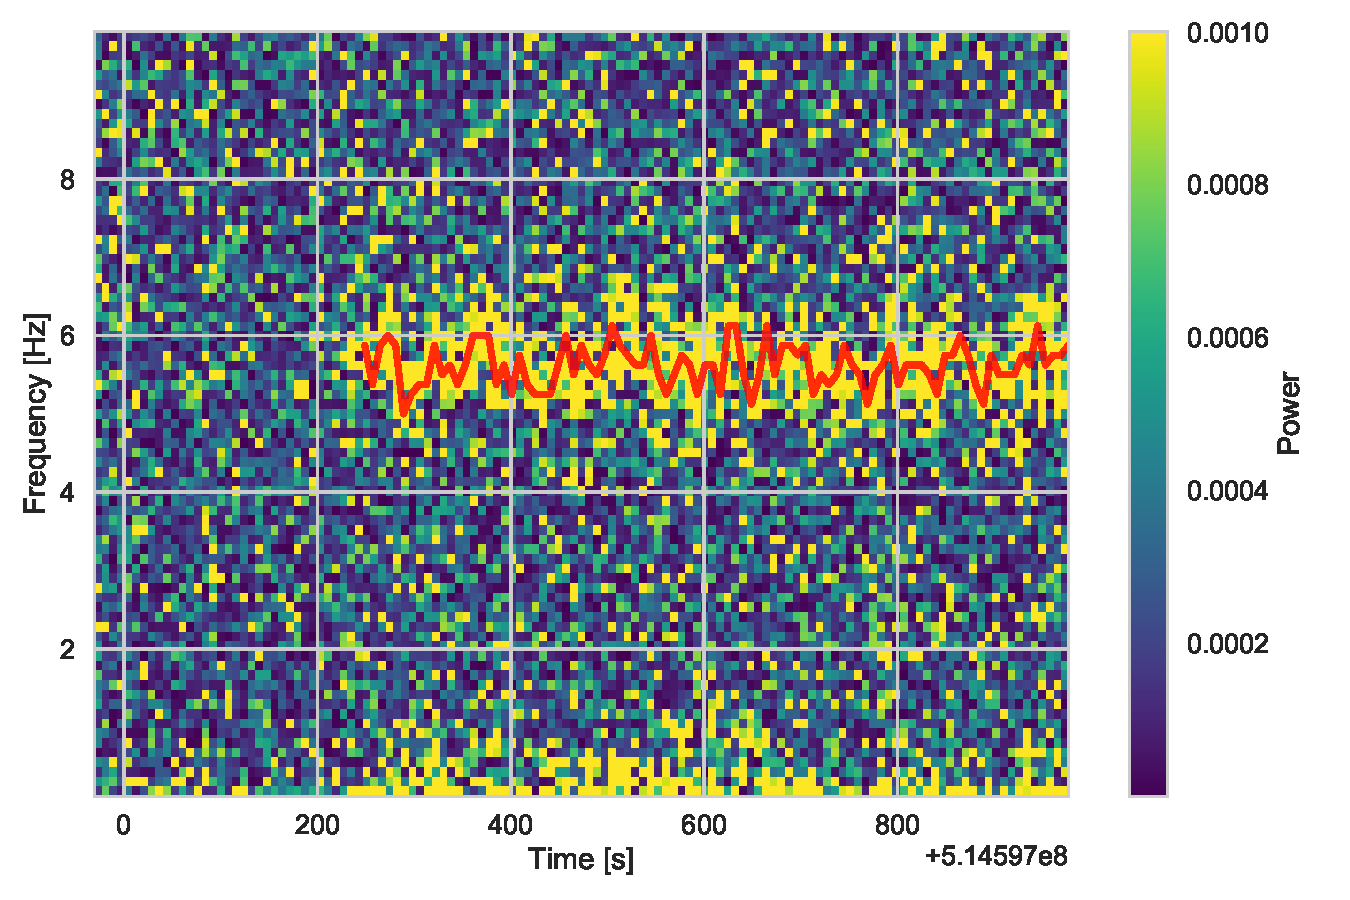
\includegraphics[width=9cm]{dyn_spec.pdf}
\caption{An example of a dynamical power spectrum. This spectrum was generated by simulating a Poisson-distributed light curve with a duration of $T=100 \mathrm{s}$, a time resolution of $dt = 0.01\,\mathrm{s}$ and an average constant count rate of $100\mathrm{counts/s}$. Superimposed on that time series is a sinusoidal signal with a frequency that itself varies around a frequency of $\nu = 25\mathrm{Hz}$ as a function of time in a periodic manner with a period of $130\,\mathrm{s}$. We split the light curve into segments of $T_\mathrm{seg} = 3\,\mathrm{s}$ duration and Fourier-transformed each individually to produce the dynamical power spectrum in this Figure. In red, we show the frequency with the highest power found in each segment, using the \mintinline{python}{trace_maximum} method.}
\label{fig:dynspec}
\end{center}
\end{figure}

For long observations with quasi-periodic oscillations (QPOs) spectrograms, more commonly known in the astronomy literature as Dynamical Power Spectra [REF], can be a useful way to track changes in the QPO centroid frequency over time. We have implemented \mintinline{python}{DynamicalPowerspectrum} as a subclass to \mintinline{python}{AveragedPowerspectrum} to provide this functionality. Like \mintinline{python}{AveragedPowerspectrum}, this class takes a \lightcurve object and a segment size as input, but instead of averaging the power spectra of each individual segment, it will create a matrix of time bins (one bin for each segment) as rows and Fourier frequencies as columns. Rebinning both along the time and frequency axis is possible. Moreover, the method \mintinline{python}{trace_maximum} automatically finds the frequency with the highest 
power in each segment and traces this maximum over time. An example using simulated data is shown in Figure \ref{fig:dynspec}.

Closely related to the cross spectrum and power spectrum are the crosscorrelation and the autocorrelation, implemented in classes \mintinline{python}{CrossCorrelation} and \mintinline{python}{AutoCorrelation}, respectively. As their respective Fourier spectra equivalents they take either one (autocorrelation) or two (cross correlation) \lightcurve objects as input and computes the correlation between the two light curves or of the single light curve with itself, along with the time lags for which the correlation was produced and the time lag at which the maximum correlation is measured.

It is useful to note that all classes in this section are compatible with Good Time Intervals

%\noindent Here, $i = \sqrt{-1}$, and $A_{xj}, A_{yj}$ and $B_{xj}, B_{yj}$ describe the real and imaginary parts of the Fourier amplitudes, respectively . We restrict $\mathcal{F}_x(j)$ and $\mathcal{F}_y(j)$ to frequencies between $\nu_{j=0} = 1/T$ and the Nyquist frequency $\nu_{j=N/2} = 1/(2\Delta t)$.
%The complex cross spectrum is then calculated by multiplying the Fourier transform of light curve $\mathbf{x}$ with the complex conjugate of the Fourier transform of light curve $\mathbf{y}$ (, see also \citealt{uttley2014} for a recent review of spectral timing techniques):




\subsection{Higher-Order Fourier Products and Spectral Timing Functionality}
\label{sec:fourier_others}

Over the past decade, higher-order Fourier products and spectral timing have emerged as key methods to study variability on different time scales as well as a function of wavelength. In \stingray, we have implemented several of the most common techniques, with plans to add to the existing tools as they become available in the future.


\section{The \texttt{modeling} Subpackage}
\label{sec:modeling}

Modelling data sets with parametric (often physically motivated) models that map an independent variable (e.g.\ time or frequency) to one or more dependent variables (e.g.\ flux, counts or Fourier powers) is a common task in astronomy. Constructing a general-purpose modelling framework is a highly non-trivial task, thus \stingray's modelling interface currently restricts itself to models of commonly used spectral-timing products, in particular modelling (averaged) power spectra. 
While it makes heavy use of the \verb|astropy.modeling.FittableModel| definitions, it does not use the fitting algorithms implemented in \texttt{astropy}. This is necessitated by the fact that the statistical properties of spectral timing products do not follow the assumptions made by the fitters implemented in \texttt{astropy}, and would thus produce incorrect results in practice.

\subsection{General Overview}
The modelling subpackage logically separates out statistical models -- likelihoods and posteriors -- from the fitting functionality, such that different likelihoods and posteriors can be straightforwardly dropped in and out depending on the data set and problem at hand\footnote{This paper is not intended as an introduction into parametric modelling and statistical inference. For suitable introductions, we recommend e.g.~ \citet{hogg2010}}. In line with the overall philosophy of \stingray, the modelling subpackage is designed to be modular and easily extensible to specific problems a user might try to solve, while many typical tasks one might do with Fourier products are already built-in. It integrates with parts of the \verb|astropy.modeling| interface, and makes use of the \verb|scipy.optimize| interface for optimization as well as the package \texttt{emcee} for Markov Chain Monte Carlo (MCMC) sampling.

\subsection{Statistical Models}

All statistical models are implemented as a subclass of an Abstract Base Class \likelihood in module \verb|stingray.posterior|. In its most basic form, each subclass of \likelihood takes data in some form (most commonly two arrays, one with the independent and one with the dependent variable) as well as an object of type \verb|astropy.modeling.FittableModel|. The likelihood itself is implemented in the \texttt{evaluate} method, which takes a set of parameters to be passed to the \verb|astropy.modeling.FittableModel| instance, computes model values for each data point in the array of independent variables and statistically compares these model values with the data points stored in the dependent variable, assuming the particular statistical distribution of the likelihood definition. The result is a single quantity, which can then be e.g.~ optimized in order to find a Maximum Likelihood (ML) solution.

For all \likelihood subclasses implemented in \stingray, there will also be an appropriate subclass of \verb|stingray.modeling.Posterior| available. As with the \likelihood subclasses, subclasses of class \verb|Posterior| take data of some form and an \verb|astropy.modeling.FittableModel| instance upon instantiation. Additionally, all subclasses of  \verb|Posterior| also require definition of a \texttt{logprior} method, which calculates the value of the prior distributions on the parameters given a particular set of parameters. There are two ways to define priors: they can be passed into the \texttt{priors} keyword argument upon instantiation of the class, or they can be set using the \verb|set_logprior| utility function in \verb|stingray.modeling|. In either case, the priors should be passed as a dictionary of \verb|"parameter name": distribution| pairs, where the parameter names match those of the \verb|astropy.modeling.FittableModel| instantiated and each distribution is a function definition that takes a parameter value and returns the probability density at that parameter value. \verb|stingray.modeling.Posterior| subclasses generally have three outward-facing methods: \verb|Posterior.logprior|, \verb|Posterior.loglikelihood| and \verb|Posterior.logposterior|. All three take a list of parameters as input. In addition, a \verb|__call__| method that executes \verb|logposterior| will allow the user to call the class instance directly and compute the log-posterior of the model given a set of input parameters. 

\verb|Loglikelihood| and \verb|Posterior| subclass definitions exist for a range of different statistical models useful in the context of astronomy data:
\begin{itemize}
\item{\verb|GaussianLogLikelihood| and \verb|GaussianPosterior| implement statistical models for data with normally distributed uncertainties. \verb|GaussianLogLikelihood| will compute what astronomers generally call $\chi^2$, because the likelihood calculated by this statistical model generally follows a $\chi^2$ distribution with $N-P$ degrees of freedom (where $N$ is the number of data points and $P$ the number of free parameters). Note, however, that this is \textbf{not} the same as the $\chi^2$ likelihood defined below!}
\item{\verb|PoissonLogLikelihood| and \verb|PoissonPosterior| calculate the likelihood and posterior for Poisson-distributed data, respectively. This likelihood is equivalent to what in astronomy is often called the \textit{Cash statistic} \citep{cash1979} and is the appropriate likelihood to use for count- or event-type data often found in X-ray astronomy time series and spectra.}
\item{\verb|PSDLogLikelihood| and \verb|PSDPosterior| implement the statistical model appropriate for modelling (averaged) power spectra, a $\chi^2$ distribution. We broke with the rule of naming likelihoods and posteriors after the statistical distribution they implement in this case, because as mentioned above, astronomers tend to call the likelihood for normally distributed data $\chi^2$, and this naming helps avoid any confusion. These two classes implement a $\chi^2_2$ distribution for Fourier spectra generated with the \powerspectrum class, and a $\chi^2_{2MK}$ distribution for power spectra generated with the \texttt{AveragedPowerspectrum} class, where $M$ is the number of averaged segments and $K$ is the number of averaged neighbouring frequency bins. Please note that as laid out in \citet{huppenkothen2017}, these distribution are \textbf{not} appropriate for use on (averaged) cross spectra. The appropriate distributions for these products will be implemented in a future version of \stingray.}
\end{itemize}

Other statistical models can be easily implemented by subclassing the \verb|LogLikelihood| and \verb|Posterior| Abstract Base Classes and using the existing classes as template..

\subsection{General Parameter Estimation and Model Comparison Functionality}

Stingray implements utility functions in order to reduce some of the overhead required for standard parameter estimation and model comparison tasks. Im particular, the \verb|parameterestimation| module implements a range of classes and functions to aid users in fitting models to data and estimating the probability distributions of parameters.

The class \verb|ParameterEstimation| provides the basis for more sophisticated, specialized implementations for particular data types. Its core methods are \verb|fit| and \verb|sample|. The former takes an instance of a \verb|LogLikelihood| or \verb|Posterior| subclass and uses minimization algorithms implemented in \verb|scipy.optimize| to find the Maximum Likelihood (ML) or Maximum-A-Posteriori (MAP) solution. The \verb|sample| method uses the Affine-Invariant MCMC sampler implemented in \verb|emcee| [REF] to generate samples from a posterior distribution passed as an instance of a subclass of \verb|Posterior|. Note that \textit{you should never pass a} \verb|LogLikelihood| \textit{instance into the} \verb|sample| \textit{method}, because sampling from a likelihood is statistically invalid. In addition to these core methods, higher-level functionality implemented in this class includes calculating the Likelihood Ratio Test (LRT) for two different models $M_1$ and $M_2$ via the \verb|compute_lrt| method (note the statistical assumptions of the LRT, and where they fail, e.g. \citealt{protassov2002}). In addition, the \verb|calibrate_lrt| method allows calibrating the p-value for rejecting the model $M_1$ via simulations of $M_1$, using either an MCMC sample (for Bayesian inference) or the covariance matrix derived from the optimization (both Bayesian and Maximum Likelihood approaches).

Stingray also implements two classes that summarize results of the optimization and sampling procedures in concise, useful ways. The \verb|fit| method returns an instance of class \verb|OptimizationResults|. This contains the most important outputs from the optimizer, but will also behind the scenes calculate a number of useful quantities, including the covariance between parameters (or a numerical approximation for some minimization algorithms), the Akaike and Bayesian Information Criteria (AIC [REF] and BIC [REF], respectively) as well as various summary statistics, e.g. the figure of merit, defined as 

\[
m = \sum_{j=1}^{N}{\left( \frac{y_j - \nu_j}{\nu_j} \right)^2} \,
\]

\noindent where $\mathbf{D} = \{x_j, y_j\}_{j=1}^{N}$ is the set of $N$ data points and $\nu_j$ is the value of the model evaluated at each $x_j$.

Similarly, an instance of class \verb|SamplingResults| is returned by the \verb|sample| method, which returns the posterior samples calculated by the MCMC sampler, as well as computes a number of helpful quantities using the MCMC chains. It calculates useful diagnostics including the acceptance fraction, the autocorrelation length and the Rubin-Gelman statistic [REF] to indicate convergence, and infers means, standard deviations and user-defined credible intervals for each parameter.

Both \verb|OptimizationResults| and \verb|SamplingResults| implement a \verb|print_results| and a \verb|plot_results| method, which produce useful text output for log files and diagnostic plots that help understand the results.

\begin{figure*}[htbp]
\begin{center}
\begin{subfigure}[b]{10.5cm}
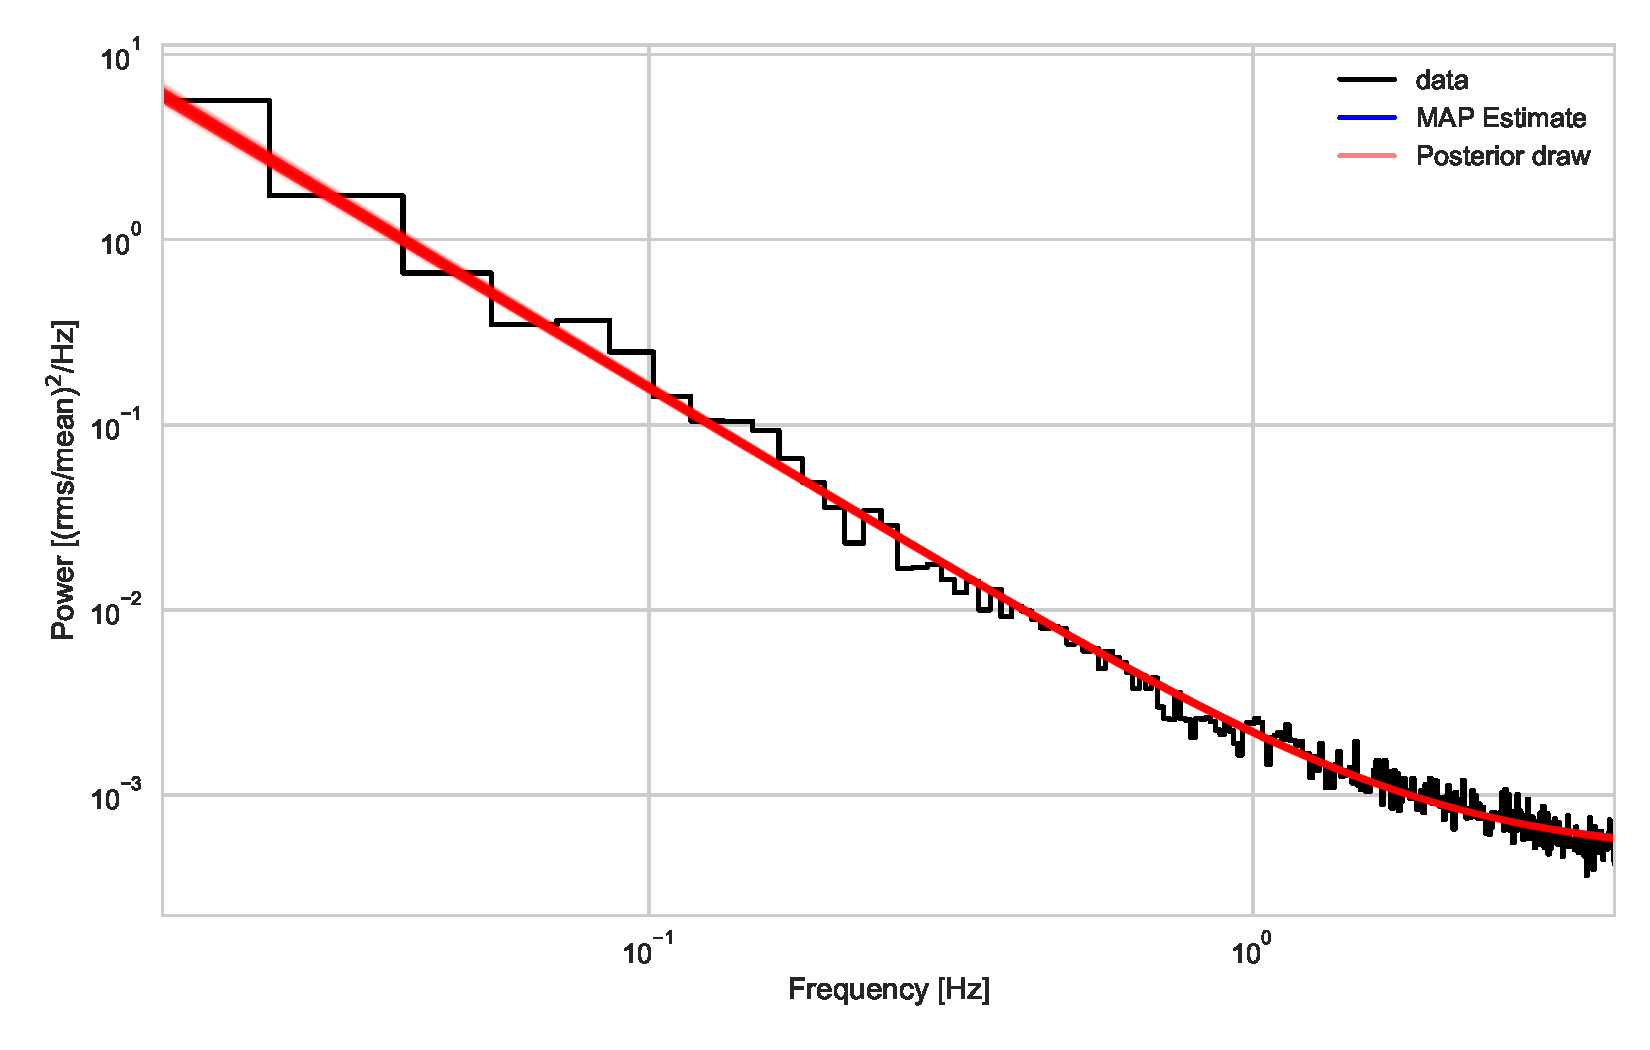
\includegraphics[width=\linewidth]{example_posterior.pdf}
\end{subfigure}
\begin{subfigure}[b]{6.8cm}
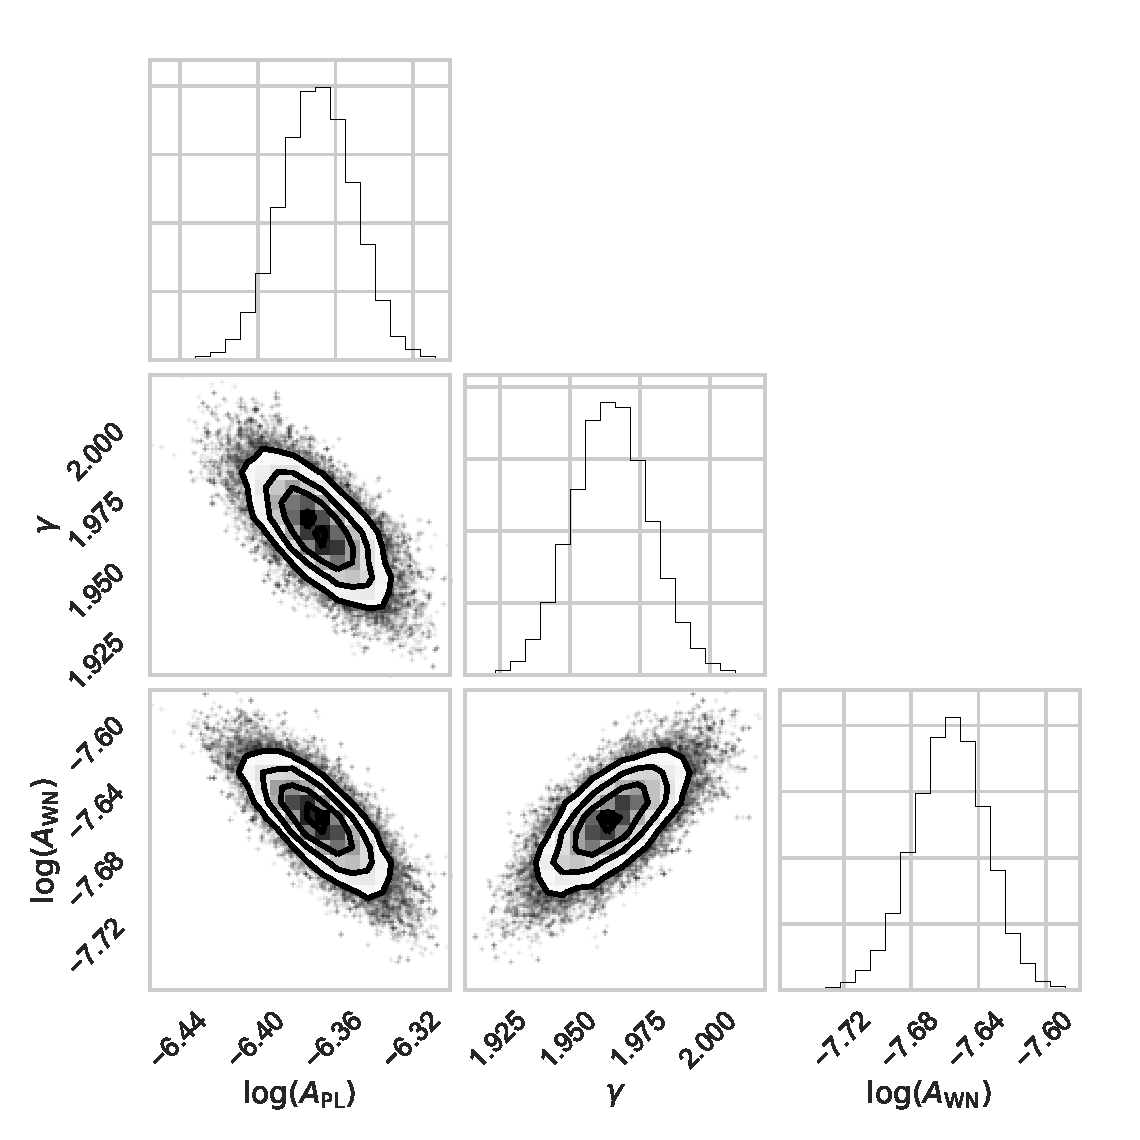
\includegraphics[width=\linewidth]{example_psd_corner.pdf}
\end{subfigure}
\caption{Left panel: The averaged periodogram from Figure \ref{fig:psd} (black), along with draws from the posterior distribution of the power law model plus constant used to model the data (red). The Maximum-A-Posteriori fit is shown in blue, but completely hidden behind the posterior draws. Right panel: corner plot showing the marginal posterior distributions (diagonal) of the three parameters of the model: the log-amplitude of the power law $A_\mathrm{PL}$, the power law index $\gamma$ and the log-amplitude of the white noise, $A_\mathrm{WN}$. The right-hand figure was produced using the package \texttt{corner} \citep{corner}.}
\label{fig:posterior}
\end{center}
\end{figure*}

\subsection{Special Functionality for Fourier Products}

The subclass \verb|PSDParEst| inherits directly from \verb|ParameterEstimation| and implements a number of additional methods particularly useful for modelling power spectra. One particularly common task is to search for periodic signals (e.g. from pulsars) in a power spectrum, which reduces to finding outliers around an assumed power spectral shape (assuming the signal is \textit{strictly} periodic, and thus all power approximately concentrated in one bin). In the presence of other variability, the probability of observing a certain power $P_j$ at a frequency $\nu_j$ under the assumption that no periodic signal is present depends on the shape and parameters of the underlying power spectral model assumed to have generated the data. As \citet{vaughan2010} show, there is an inherent uncertainty in our inference of the parameters of this power spectral model, which must be taken into account via simulations. \verb|PSDParEst| implements a method \verb|calibrate_highest_outlier|, which finds the $k$ highest outliers (where $k$ is a user-defined number) and calculates the posterior predictive $p$-value that said outlier can be explained by noise only. It makes heavy use of the method \verb|simulate_highest_outlier|, which uses the \verb|sample| method to derive an MCMC sample and then simulate fake power spectra from that model for a range of plausible parameter values in order to include our model uncertainty into the $p$-value. For details of the overall procedure, see \citet{vaughan2010}. 

As of this version, the \verb|stingray.modeling| subpackage has no functionality to model higher-order Fourier products. For spectral timing in particular, this would involve being able to read and apply instrument responses to models, as well as being able to interface with the library of spectral models associated with the X-ray spectral fitting tool XSPEC \citep{arnaud1996}. Providing this functionality is planned for a future release of \stingray. 

For an example workflow describing how to model a power spectrum using \stingray, see [ADD CODE].


\begin{listing}
\begin{minted}
[frame=lines,
framesep=2mm,
baselinestretch=1.2,
bgcolor=white,
fontsize=\footnotesize,
linenos
]{python}
from scipy.stats import uniform
from astropy.modeling import models
from stingray import sampledata
from stingray import Lightcurve
from stingray import Powerspectrum, AveragedPowerspectrum
from stingray.modeling import PSDPosterior, PSDParEst
from stingray.modeling import set_logprior

# load light curve 
lc = sampledata.sample_data() 

# create a PSD
ps = Powerspectrum(lc, norm="frac")

# compute averaged power spectrum
avg_ps = AveragedPowerspectrum(lc, 
                               segment_size=64, 
                               norm="frac")

# create a model instance
m = models.PowerLaw1D() + models.Const1D()
m.x_0_0.fixed=True

# create the posterior object
lpost = PSDPosterior(freq=avg_ps.freq, 
                     power=avg_ps.power, 
                     model=m, 
                     m=avg_ps.m)

# set priors
amp_prior = lambda amp: uniform(-15, 30).pdf(np.log(amp))
alpha_prior = lambda alpha: uniform(0,5).pdf(alpha)
priors = {"amplitude_0":amp_prior, 
          "alpha_0":alpha_prior,
          "amplitude_1": amp_prior}

lpost.logprior = set_logprior(lpost, priors)

# create ParameterEstimation object
parest = PSDParEst(avg_ps, fitmethod="BFGS", 
             max_post=True)

# fit using optimization
res = parest.fit(lpost, [0.005, 2, 0.001])

# MCMC sampling
sample = parest.sample(lpost, res.p_opt, 
                       cov=res.cov, 
                       nwalkers=250, 
                       niter=200, burnin=1000, 
                       threads=1)

\end{minted}
\caption{A typical workflow for modelling (averaged) power spectra.The results can be found in Figure \ref{fig:posterior}.}
\label{list:modeling}
\end{listing}

\section{The \texttt{simulator} Subpackage}
\label{sec:simulator}

\section{The \texttt{pulse} Subpackage}
\label{sec:pulsar}
\stingray contains the basic operations to perform the search and characterization of pulsed signals.
(...)
\subsection{Folding}
Among the basic algorithms used in pulsar astronomy, one cannot overstate the importance of Epoch Folding (EF).
The algorithm consists of cutting the signal at every pulse period and summing all sub-intervals in phase. 
An alternative way of seeing it, more useful for photon data, is just a \textit {histogram of pulse phases}.

If the period is exactly correct and assuming a stable pulsation, the signal-to-noise ratio will get better approximately with the square root of the number of summed sub-intervals [REF].
This is the method used to obtain practically all pulse profiles shown in the literature, as most pulsar signals are orders of magnitude below noise level.

The `pulse.pulsar` submodule contains the functionality to calculate the phase given a simple pulse ephemeris consisting of any number of pulse frequency derivatives%
\footnote{For more complicated cases, like binary pulsars or long-term pulsar noise not well described by pulse derivatives, we recommend to look at more focused libraries like \href{https://github.com/nanograv/PINT}{PINT} [REF]}.
Moreover, we have a mechanism to calculate the exposure of single bins in the pulse profile. 
This is particularly useful for very long-period pulsars where the pulsed period is comparable to the length of the GTIs.
The different exposure of pulse bins caused by the absence of signals during GTIs is taken into account in the calculation of the final pulse profile by the folding algorithm, if the user asks for it. 

\subsection{Epoch Folding and \zsq search}
\label{sec:efzsq}
During a search for pulsations, the first step is usually the PDS. 
However, often pulsations do not leave a clear signature above noise level in the PDS, because they are weak or they fall close to bin edges, where the sensitivity is reduced [REF].
Even when they do, the frequency resolution of the PDS is often inadequate to measure precisely the pulse frequency.
Therefore, an additional statistical analysis is needed. 
In this Section, we will describe the Epoch Folding search (EFS).
This search method consists of executing the folding at many trial frequencies around the candidate frequency.
Once the folding is performed, the following statistics is calculated on the profile:
\begin{equation}
\mathcal{S} = \sum_i\frac{(P_i - \overline{P})^2}{\sigma^2}
\end{equation}
where $P_i$ are the bins of the profile, $\overline{P}$ is the mean level of the profile, and $\sigma$ is the standard deviation.
This is the \textit{chi squared} of the actual pulsed profile with respect to a \textit{flat} model.

If there is no pulsation, the chi squared will assume a random value distributed around the number of degrees of freedom $n - 1$ (where $n$ is the number of bins in the profile) with a well defined statistical distribution ($\chi^2_{n - 1}$) that allows an easy calculation of detection limits. 
When a peak is \textit{very unlikely} (meaning that the probability to be obtained by noise is below a certain $\epsilon$), this peak is considered a pulse candidate.
If the frequency resolution is sufficiently high, close to the correct frequency, as described by [Leahy et al. 1983, 1987], the peak in the epoch folding periodogram has the shape of a \textbf{sinc squared function} whose width is driven by the length of the observation.

The epoch folding statistics, however, can give the same value for a pulse profile at the correct frequency and, for example, an harmonic that produces a deviation from a Poisson distribution.
A more effective method is the $Z^2_n$ statistics (Buccheri et al. 1983), which is conceptually similar to EF but has high values when the signal is well described by a small number of \textbf{sinusoidal harmonics}: 

\begin{equation}
\zsq = \dfrac{2}{N} \sum_{k=1}^n \left[{\left(\sum_{j=1}^N \cos k \phi_j\right)}^2 + {\left(\sum_{j=1}^N \sin k \phi_j\right)}^2\right]
\end{equation}

Where $N$ is the number of photons, $n$ is the number of harmonics, $\phi_j$ are the phases corresponding to the event arrival times $t_j$ ($\phi_j = \nu t_j$, where $\nu$ is the pulse frequency).

The \zsq statistics defined in this way, far from the pulsed profile, follows a $\chi^2_n$ distribution, where $n$ is the number of harmonics this time.
This allows, again, to easily calculate thresholds based on the probability of obtaining a given \zsq by pure noise.

The standard \zsq search calculates the phase of each photon and calculates the sinusoidal functions above for each photon.
This is very computationally expensive if the number of photons is high. 
Therefore, in Stingray, the search is performed by binning the pulse profile first and using the phases of the folded profile in the formula above, multiplying the squared sinusoids of the phases of the pulse profile by a weight corresponding to the number of photons at each phase.

\begin{equation}
\zsq \approx \dfrac{2}{\sum_j{w_j}} \sum_{k=1}^n \left[{\left(\sum_{j=1}^m w_j \cos k \phi_j\right)}^2 + {\left(\sum_{j=1}^m w_j \sin k \phi_j\right)}^2\right]
\end{equation}

Since the sinusoids are only executed on a small number of bins, while the epoch folding procedure just consists of a very fast histogram-like operation, the speedup of this new formula is obvious. 
Care must be put into the choice of the number of bins, in order to maintain a good approximation even when the number of harmonics is high. 
We recommend in the documentation to use a number of bins at least 10 times larger than the number of harmonics.

\subsection{Characterization of pulsar behavior}
\label{sec:ephem}
As seen in Section~\ref{sec:efzsq}, the \zsq or the EF periodograms of a perfectly stable pulsation have the shape of a sinc squared function.
\stingray has additional functionality to fit these periodograms with sinc squared or Gaussian models, and find the mean frequency with high precision.

A significant deviation from the expected shape from these peaks in the periodogram can happen if the pulsation is not stable.
Calculating the periodogram is an option to investigate how the pulse phase varies in time.
The periodogram is basically a 2-D histogram of the phase and arrival times of the pulses. 
If the pulsation is stable and the pulse frequency was determined with precision, the periodogram shows vertical stripes corresponding to perfectly aligned pulses.
If the frequency is not as precise, the stripes become more and more diagonal.
If the pulse has a detectable frequency derivative, these stripes bend with a parabolic shape.

A very precise way to determine the exact pulse ephemeris is out of the scope of \stingray. 
However, \stingray has a mechanism to calculate the pulse arrival times (or times of arrival, TOAs) using a pulse template, using the \texttt{fftfit} algorithm used for radio pulsars. 
This is implemented in the \verb|get_TOA| function in `stingray.pulse.pulsar`.
Then, the user can use the TOAs with more focused software like Tempo, Tempo2 or PINT.

[Fig. XXXX: a variation of the pulse phase corresponding to a period derivative. ]

\section{Connections to \texttt{DAVE}}
\label{sec:dave}

\section{\hendrics: command-line interface}
\label{sec:hendrics}


\section{Development and Integration Environment}
\label{sec:development}

\section{Future Development Plans}
\label{sec:future}

\paragraph{acknowledgements}
DH acknowledges support from the DIRAC Institute in the Department of Astronomy at the University of Washington. The DIRAC Institute is supported through generous gifts from the Charles and Lisa Simonyi Fund for Arts and Sciences, and the Washington Research Foundation.
We thank Astro Hack Week for providing the venue that started this project and the Lorentz Centre for organizing the workshop that started the collaboration. We thank the Google Summer of Code Program for funding a total 5 students who implemented a large fraction of the various library components over two summers.

\bibliography{stingraypaper}
\bibliographystyle{apj}

\end{document}


